\documentclass[border=2pt]{standalone}
\usepackage{tikz}
\usetikzlibrary{arrows.meta}
\begin{document}
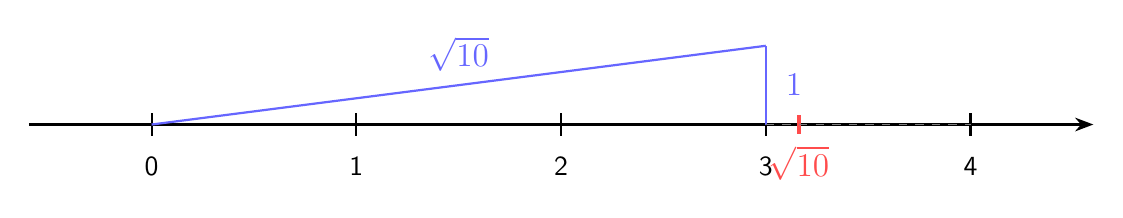
\begin{tikzpicture}[x=2.6cm, y=1cm, font=\sffamily]
  % garis bilangan utama
  \draw[thick, -{Stealth}] (-0.6,0) -- (4.6,0);
  % titik bilangan bulat 0..4 dengan label di bawah
  \foreach \x in {0,...,4} {
    \draw[thick] (\x,0.14) -- (\x,-0.14) node[below=4pt] {\x};
  }
  % segitiga siku-siku: kaki 3 dan 1, sisi miring sqrt(10)
  \draw[thick, blue!60] (3,0) -- (3,1);
  \draw[thick, blue!60] (0,0) -- (3,1);
  \node[above, blue!60] at (1.5,0.55) {\large $\sqrt{10}$};
  \node[right, blue!60] at (3.05,0.5) {\large $1$};
  % tanda potong di garis bilangan pada sqrt(10) ~ 3.16
  \draw[very thick, red!70] ({sqrt(10)},-0.12) -- ({sqrt(10)},0.12);
  \node[below, red!70] at ({sqrt(10)},-0.15) {\large $\sqrt{10}$};
  % penanda sementara antara 3 dan 4
  \draw[dashed, gray] (3,0) -- (4,0);
\end{tikzpicture}
\end{document}
